\chapter{绪论}\label{cha:introduction}

\section{研究背景及意义}
\subsection{古早计算机}
本来,计算机的英文原词``computer''是指从事数据计算的人。而他们往往都需要借助某些机械计算设备或模拟计算机。

这些早期计算设备的祖先包括有算盘,以及可以追溯到公元前87年的被古希腊人用于计算行星移动的安提基特拉机械。随着中世纪末期欧洲数学与工程学的再次繁荣,1623年德国博学家Wilhelm Schickard率先研制出了欧洲第一部计算设备,這是一個能進行六位以內數加減法,並能通過鈴聲輸出答案的“計算鐘”。使用轉動齒輪來進行操作。

1642年法國數學家布莱士·帕斯卡在英国数学家William Oughtred所制作的“計算尺”的基礎上,將其加以改進,使能進行八位計算。還賣出了許多製品,成為當時一種時髦的商品。

\subsection{近代计算机}
1801年,法国人约瑟夫·玛丽·雅卡尔对织布机的设计进行改进,使用一系列打孔的纸卡片来作为编织复杂图案的程式。尽管这种被称作“雅卡尔织布机”的机器并不被认为是一部真正的计算机,但是其可程式化性质使之被视为现代计算机发展过程中重要的一步。

查尔斯·巴貝奇于1820年构想和设计了第一部完全可程式化计算机。但由于技术条件、经费限制,以及无法忍耐对设计不停的修补,这部计算机在他有生之年始终未能问世。约到19世纪晚期,许多后来被证明对计算机科学有着重大意义的技术相继出现,包括打孔卡片以及真空管。德裔美籍统计学家赫爾曼·何樂禮设计了一部制表用的机器,其中便应用打孔卡片来进行大规模自动数据处理。



\subsubsection{小节}
试一下引用\cite{Li_2020},(见\autoref{fig:lengthscale})。

\begin{figure}[htbp]
  \centering
  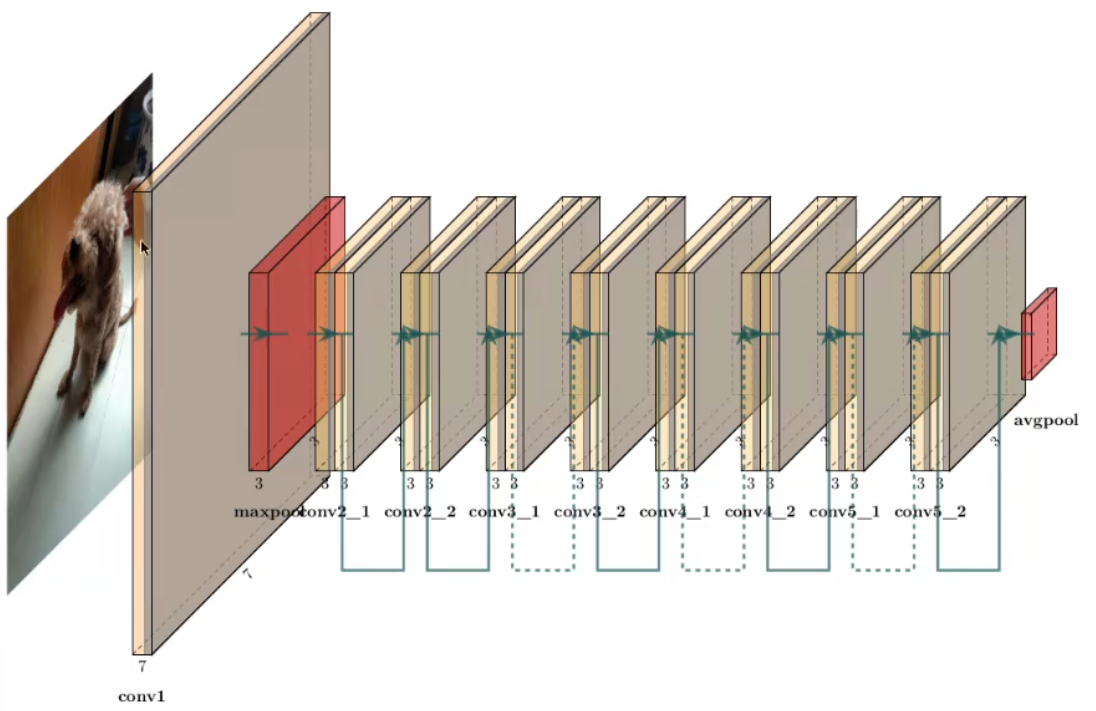
\includegraphics[width=0.8\textwidth]{figures/introduction/RESNet18.png} \\
  \caption[ResNet18网络结构示意图]{ResNet18是一个深度卷积神经网络结构} 
  \label{fig:lengthscale}
\end{figure}

本章是第~\ref{cha:introduction}~章。下一节是~\ref{sec:challenge}。
